\documentclass[british]{article}
\usepackage[T1]{fontenc}
\usepackage[utf8]{luainputenc}
\usepackage[a4paper]{geometry}
\geometry{verbose,tmargin=2cm,bmargin=2cm,lmargin=2cm,rmargin=2cm}
\usepackage{fancyhdr}
\pagestyle{fancy}
\setcounter{tocdepth}{2}
\usepackage{xcolor}
\usepackage{babel}
\usepackage{multirow}
\usepackage{graphicx}
\usepackage{setspace}
\usepackage{microtype}
\onehalfspacing
\usepackage[unicode=true,pdfusetitle,
 bookmarks=true,bookmarksnumbered=true,bookmarksopen=false,
 breaklinks=false,pdfborder={0 0 0},pdfborderstyle={},backref=section,colorlinks=false]
 {hyperref}
\makeatletter
\providecommand{\tabularnewline}{\\}
\@ifundefined{date}{}{\date{}}
\usepackage{array}
\usepackage{multirow}
\providecommand{\tabularnewline}{\\}
\usepackage{multirow}
\AtBeginDocument{
  \def\labelitemi{\large\(\star\)}
}
\usepackage{babel}
\fancyhead[RO]{\textsl{TABLE OF CONTENTS}}
\fancyhead{}
\fancyhead[RE,LO]{\leftmark}

\AtBeginDocument{
  \def\labelitemi{\large\(\star\)}
}

\makeatother

\begin{document}
\medskip{}

\title{\textbf{\Huge{}LECTURE NOTES ON DIGITAL FORENSICS}{\Huge{}\vfill{}
	}Digital Forensics}
\author{{\LARGE{}\vspace{1.5cm}
		}\textbf{\LARGE{}AGNI DATTA}}
\maketitle
\begin{center}
	{\LARGE{}\vfill{}
	}{\LARGE\par}
	\par\end{center}

\begin{center}
	{\Huge{}\rule[0.5ex]{0.5\columnwidth}{0.5pt}}{\Huge\par}
	\par\end{center}

\begin{center}
	{\LARGE{}Lecture Notes collected from classes of Dr. Shishir Kumar
		Shandilya}\\
	{\LARGE{} DIGITAL FORENSICS}{\LARGE\par}
	\par\end{center}

\begin{center}
	{\LARGE{}\vfill{}
	}{\Large{}SCHOOL OF COMPUTER SCIENCE}\\
	{\Large{} VELLORE INSTITUTE OF TECHNOLOGY}\\
	{\Large{} \vfill{}
	}\pagebreak\tableofcontents{}
	\par\end{center}

\newpage{}

\part{Introduction to Digital Forensics:}

Digital forensics is the use of scientifically derived and proven
methods towards the preservation, collection, validation, identification,
analysis, interpretation, documentation and presentation of digital
evidence derived from digital sources for the purpose of facilitating
the reconstruction of events found to be criminal, or helping to anticipate
unauthorized actions shown to be disruptive to planned operations.
It involves the application of investigation and analysis techniques
to gather and preserve evidence from a particular computing device
in a way that is suitable for presentation in a court of law. The
goal of computer forensics is to perform a structured investigation
while maintaining a documented chain of evidence to find out exactly
what happened on a computing device and who was responsible for it.

\rule[0.5ex]{0.75\columnwidth}{1pt}

\section{Importance of Computer Forensics:}

The computer has invaded our very existence, become a part of our
lives, and is an integral part of almost every case. Computer Forensics
can help any organization in finding evidence in a variety of cyber
crime cases. Crimes involving a computer can range across the spectrum
of criminal activity, from child pornography to theft of personal
data to destruction of intellectual property. Computer Forensics not
only means recovering deleted files (documents, graphics, etc.), but
also searching the slack and unallocated space on the hard drive-places
where a plethora of evidence regularly resides. It is tracing Windows
artefacts- those titbits of data left behind by the operating system-for
clues of what the computer has been used for, and, more importantly,
knowing how to find the artefacts, and evaluating the value of information.
Forensic exams allow the processing of hidden files-files that are
not visible or accessible to the user-that contain past usage information.
It is reconstructing and analysing the date codes for each file-determining
when each file was created, last modified, last accessed and when
deleted. Computer forensics is being able to run a string-search for
e-mail, when no e- mail client is obvious. An analysis will reveal
Internet usage, recover data, and accomplish a full analysis even
after the computer has been formatted. It is using industry-standard
methodology, and with a concise report with clearly demonstrable results,
something that is organized in a manner to make analysis easier.

\rule[0.5ex]{0.75\columnwidth}{1pt}

\section{Locard\textquoteright S Exchange Principle:}

Dr. Edmond Locard (13 December 1877 -- 4 April 1966) was a pioneer
in forensic science who became known as the \textquotedbl Sherlock
Holmes of France\textquotedbl . He formulated the basic principle
of forensic science: \textquotedbl\textcolor{red}{Every contact leaves
	a trace}\textquotedbl .

This became known as Locard's exchange principle. ``\textcolor{red}{Anyone,
	or anything that enters in the crime scene takes something from the
	crime scene with them and leaves something behind, and that both can
	be used as forensic evidence}''. Crime reconstruction involves examining
the available physical evidence, those materials left at or removed
from the scene, victim, or offender, for example fingerprints. These
forensically established contacts are then considered in light of
available and reliable witness, the victim, and a suspect's statements.
From this, theories regarding the circumstances of the crime can be
generated and falsified by logically applying the information of the
established facts of the case.

\rule[0.5ex]{0.75\columnwidth}{1pt}

\section{Cardinal Rules of Digital Forensics:}

\paragraph{Following are the cardinal rules of the Digital Forensics:}
\begin{itemize}
	\item Never mishandle the evidence.
	\item Never trust the subject machine or Operating system.
	\item Never work on the original evidence.
\end{itemize}
\rule[0.5ex]{0.75\columnwidth}{1pt}

\section{Digital Evidence:}

Digital evidence is defined as information and data of value to an
investigation that is stored on, received or transmitted by an electronic
device. This evidence can be acquired when electronic devices are
seized and secured for examination.

Digital evidence:
\begin{itemize}
	\item Is latent (hidden), like fingerprints or DNA evidence,
	\item Crosses jurisdictional borders quickly and easily,
	\item Can be altered, damaged or destroyed with little effort,
	\item Can be time sensitive.
\end{itemize}
\begin{description}
	\item [{Admissibility:}] Digital evidence is often ruled inadmissible by
	      courts because it was obtained without authorization. In most jurisdictions
	      a warrant is required to seize and investigate digital devices. In
	      a digital investigation this can present problems where, for example,
	      evidence of other crimes are identified while investigating another.
	      Authentication: As with any evidence, the proponent of digital evidence
	      must lay the proper foundation. Courts largely concerned themselves
	      with the reliability of such digital evidence. Best evidence rule
	      is a legal principle that holds an original copy of a document as
	      superior evidence. The rule specifies that secondary evidence, such
	      as a copy or facsimile, will be not admissible if an original document
	      exists and can be obtained. \textquotedbl Secondary evidence\textquotedbl{}
	      or copies of the content in the original document can be admitted
	      as evidence. The best evidence rule is only applied in situations
	      in which a party attempts to substantiate a non-original document
	      submitted as evidence during a trial. Admissibility of documents before
	      state court systems may vary.
\end{description}
Digital Evidence should be the following:
\begin{itemize}
	\item Admissible: Conform to legal requirements,
	\item Authentic: Relevant to the case,
	\item Complete: Not just extracts
	\item Reliable: Collected and Handled appropriately,
	\item Believable and understandable.
\end{itemize}

\subsection{Legal Issues:}

MAC details of the files as digital evidence in the seized original
hard disk (hence its image too) must be earlier than the noticing
/ reporting of criminal incident as well as the date \& time of its
seizure. If it is not so, digital evidence will be diagnosed as a
tampered evidence and court can not accept it as an admissible evidence.

\subsection{Types of Digital Evidence:}

\subsubsection{Volatile (Non-persistent) Memory that loses its contents, as soon
	as power is turned off; e.g. Data stored in RAM (semiconductor storage)
	(System BIOS: CMOS RAM - battery powered) }

\subsubsection{Non-volatile (Persistent) No change in contents, even if power is
	turned off; e.g. Data stored in a tape / hard disk (magnetic storage),
	CD / DVD (optical storage), data cards, USB Thumb Drives -- Flash
	memory).}

\subsection{Order of Volatility:}

Higher Volatility to Lower Volatility List:
\begin{enumerate}
	\item Registers \& Cache
	\item Routing Tables
	\item ARP Cache
	\item Process Table
	\item Kernel Statistics \& Modules
	\item Main Memory (RAM)
	\item Temporary System files
	\item Secondary Memory
	\item Router Configuration
	\item Network Topology
\end{enumerate}

\subsection{Importance of Order of Volatility:}

Current running state and system configuration details.
\begin{itemize}
	\item Activities performed/ In progress
	\item Root cause of the incident
	\item Timeline of the incident
	\item Time, date, user responsible for the incident
	\item Network connection details
\end{itemize}
Once system is shutdown / rebooted volatile data is lost for ever.

\rule[0.5ex]{0.75\columnwidth}{1pt}

\section{Procedure of Collecting Digital Evidence:}

\subsection{Order of Handling Data In Crime Scene:}
\begin{itemize}
	\item Document the Crime Scene - OS (Version),
	\item BIOS date \& time (and difference, if any),
	\item H/W and S/W Configuration,
	\item IP / MAC address,
	\item Computer System : Shutdown / Power Off ?
	\item Identify Evidence \& Authenticate through a Hashing Algorithm (MD5),
	\item Always make the bit-stream copy (forensic image) of the seized storage
	      media,
	\item Label all the connecting cables and photograph them,
	\item Document the chain of custody,
	\item Preserve the evidence before packing for transportation,
	\item Securely pack \& transport the evidence to lab,
	\item Store the seized evidence in a protected storage (air bubbled PVC,
	      anti-static bag),
	\item Transfer the Computer System to a secure location.
\end{itemize}

\subsubsection{Document Everything:}

The Crime Scene Computer forensics is a meticulous practice. When
a crime involving electronics is suspected, a computer forensics investigator
takes each of the following steps to reach --- hopefully --- a successful
conclusion: Secure the area, which may be a crime scene. Document
the chain of custody of every item that was seized. If someone is
already working on the system then ask/ insist him/her to leave the
terminal. Take photographs, note down the important things, if any.
Bag, tag, and safely transport the equipment and e-evidence. Acquire
the e-evidence from the equipment by using forensically sound methods
and tools to create a forensic image of the e-evidence. Keep the original
material in a safe, secured location. Design your review strategy
of the e-evidence, including lists of keywords and search terms. Examine
and analyse forensic images of the e-evidence (never the original!)
according to your strategy. Interpret and draw inferences based on
facts gathered from the e-evidence. Describe your analysis and findings
in an easy-to-understand and clearly written report. Give testimony
under oath in a deposition or courtroom.

\subsubsection{Securing The Crime Scene:}

Secure the area containing the equipment or the crime scene. Secure
the entrances and exits to the digital scene. Move people away from
computer and power supply as it may lead to contamination if anyone
touches anything. Preventing changes in potential digital evidence,
including network isolation, collecting volatile data, and copying
entire digital environment is the goal of this phase. If there are
any ongoing processes, they have to be captured so that to not cause
loss of potential evidence.

\subsubsection{Identifying The Evidence Sources:}

Generating a plan of action to conduct an effective digital investigation,
and obtaining supporting resources and materials is a part of this
phase. Recognizing an incident from indicators and determining its
type, which entails the preparation of tools, techniques, search warrants,
and monitoring authorizations and management support. Finding potential
sources of digital evidence (e.g., at a crime scene, within an organization,
or on the Internet) is done.

\paragraph{What should be seized for the retrieval of evidence?}

\subparagraph{Examples:}
\begin{itemize}
	\item Main unit, usually the box to which the monitor and keyboard are attached.
	\item Monitor, keyboard and mouse (only necessary in certain cases.)
	\item Power supply units.
	\item Hard disks not inside the computer.
	\item Dongles
	\item Modems (some contain phone numbers).
	\item External drives and other external devices.
	\item Routers.
	\item Digital cameras.
	\item Back up tapes.
	\item CDs/ DVDs.
	\item Memory sticks, memory cards and all USB connected devices.
\end{itemize}

\subsubsection{Document The Scene:}

Photographs or videos of digital evidence are taken individually as
well as crime scene and individuated descriptions of digital evidences
are to be made. Each piece of digital evidence that is found during
the analysis of the image must be clearly documented. Proper thorough
chain of custody has to be maintained. Chain of custody is a form
which documents the movement of evidence from its source to when it
is presented in court.

It is essential that any items of evidence can be traced from the
crime scene to the court room, and everywhere in between, known as
\textcolor{red}{CHAIN OF CUSTODY}.
\begin{itemize}
	\item Positive control is the phrase most often used to describe the standard
	      of care taken in the handling of potential evidentiality material
	      (e.g., suspect computer systems, hard drives, and any backup copies).
	\item Who handled the evidence?
	\item What procedures were performed on the evidence?
	\item When was the evidence collected and/or transferred to another party?
	\item Where was the evidence collected and stored?
	\item How was the evidence collected and stored?
	\item For what purpose was the evidence collected?
\end{itemize}

\subsubsection{Acquire The Evidence:}

Analysis should always take place on a forensically sound copy, or
image, of the seized data, rather than the original data itself. For
this purpose a bit by bit copy of the evidence is to be made. The
storage device is first connected to a ``write blocking'' device,
which prevents any binary code from being altered or modified during
the process. Then a mirror image or ``clone'' of the drive is created
on a separate storage device to be examined later. During the acquisition
process, such software creates a unique numerical code, called a verification
``hash'' of the media, which allows an analyst to later confirm
that the image and its contents are accurate and unaltered. Data acquisition
can be carried out either online (live) or offline (dead). A dead
acquisition is carried out without the support of the suspect's operating
system while a live acquisition is carried out with the support of
suspect operating system.

\subsubsection{Photography and Videography:}

Forensic photography, also referred to crime scene photography, is
an activity that records the initial appearance of the crime scene
and physical evidence, in order to provide a permanent record for
the courts and for the record. Proper documentation is to be done
and the evidences , the crime scene is to be photographed with a view
to properly locate the things in and around the vicinity of the crime
scene.

The following details/ steps need to be photographed sequentially
with proper scale and labelling: When entering the scene of crime,
photograph the scene to record the details of the crime scene. Photograph
the live status of the system found at the scene, this includes current
applications opened, cables/ USB attached, any running processes etc.
After collection, the evidence is photographed with and without a
scale and before and after packaging.

\rule[0.5ex]{0.75\columnwidth}{1pt}

\section{Communities\textquoteright{} Works in Digital Forensics:}

\paragraph{Communities working in Digital Forensics:}
\begin{itemize}
	\item Law Enforcement (i.e. Police)
	\item Military/Intelligence
	\item Business \& Industry
	\item Academia/Researchers
\end{itemize}
\rule[0.5ex]{0.75\columnwidth}{1pt}

\vfill{}


\section{Uses of Digital Forensics:}

\paragraph*{Digital forensics can be used in a variety of settings, including}
\begin{itemize}
	\item Criminal Investigations
	\item Civil Litigation
	\item Intelligence
	\item Administrative Matters
\end{itemize}

\subsection{Criminal Investigation:}

\paragraph{In today\textquoteright s digital world, electronic evidence can
	be found in almost any criminal investigation conducted. }
\begin{itemize}
	\item Homicide, physical assault, robbery, and burglary are just a few of
	      the many examples of ``analogue'' crimes that can leave digital
	      evidence.
	\item One of the major struggles in law enforcement is to change the paradigm
	      of the police and get them to think of and seek out digital evidence.
	\item Everyday digital devices such as cell phones and gaming consoles can
	      hold a treasure trove of evidence.
	\item Unfortunately, none of that evidence will ever see a courtroom if
	      it's not first recognized and collected.
	\item As time moves on and our law enforcement agencies are replenished
	      with ``younger blood,'' this will become less and less of a problem.
\end{itemize}

\subsection{Civil Litigation:}

Civil litigation is a legal process in which criminal charges and
penalties are not at issue. When two or more parties become embroiled
in such a non-criminal legal dispute, the case is presented at a trial
where plaintiffs seek compensation or other damages from defendants.

The use of digital forensics in civil cases is big business. In 2011,
the estimated total worth of the electronic discovery market is somewhere
north of \$780 million (Global EDD Group). As part of a process known
as Electronic Discovery (e-Discovery), digital forensics has become
a major component of much high dollar litigation. e-Discovery ``refers
to any process in which electronic data is sought, located, secured,
and searched with the intent of using it as evidence in a civil or
criminal legal case'' In a civil case, both parties are generally
entitled to examine the evidence that will be used against them prior
to trial. This legal process is known as ``discovery.'' Previously,
discovery was largely a paper-based exercise, with each party exchanging
reports, letters, and memos; however, the introduction of digital
forensics and e-Discovery has greatly changed this practice. The proliferation
of the computer has rendered that practice nearly extinct. Today,
parties no longer talk about filing cabinets, ledgers, and memos;
they talk about hard drives, spreadsheets, and file types. Some paper-based
materials may come into play, but it's more the exception than the
rule. Seeing the evidentiality landscape rapidly changing, the courts
have begun to modify the rules of evidence. The rules of evidence,
be they state or federal rules, govern how digital evidence can be
admitted during civil litigation. The Federal Rules of Civil Procedure
were changed in December 2006 to specifically address how electronically
stored information is to be handled in these cases. Digital evidence
can quickly become the focal point of a case, no matter what kind
of legal proceeding it's used in. The legal system and all its players
are struggling to deal with this new reality.

\subsection{Intelligence:}
\begin{itemize}
	\item Terrorists and foreign governments, the purview of our intelligence
	      agencies, have also joined the digital age.
	\item Terrorists have been using information technology to communicate,
	      recruit, and plan attacks.
	\item The armed forces are exploiting intelligence collected from digital
	      devices brought straight from the battlefield.
	\item This process is known as DOMEX (Document and Media Exploitation).
	\item DOMEX is paying large dividends, providing actionable intelligence
	      to support the soldiers on the ground army.
\end{itemize}

\subsection{Administrative Matters:}
\begin{itemize}
	\item Digital evidence can also be valuable for incidents other than litigation
	      and matters of national security.
	\item Violations of policy and procedure often involve some type of electronically
	      stored information, for example, an employee operating a personal
	      side business, using company computers while on company time.
	\item That may not constitute a violation of the law, but it may warrant
	      an investigation by the company.
\end{itemize}
\rule[0.5ex]{0.75\columnwidth}{1pt}

\vfill{}


\section{Role of The Forensic Examiner in The Judicial System:}
\begin{itemize}
	\item The digital forensics practitioner most often plays the role of an
	      expert witness.
	\item What makes them different than non expert witnesses? Other witnesses
	      can only testify to what they did or saw. They are generally limited
	      to those areas and not permitted to render an opinion.
	\item Experts, by contrast, can and often do give their opinion. What makes
	      someone an ``expert?'' In the legal sense, it's someone who can
	      assist the judge or jury to understand and interpret evidence they
	      may be unfamiliar with.
	\item To be considered an expert in a court of law, one does not have to
	      possess an advanced academic degree.
	\item An expert simply must know more about a particular subject than the
	      average lay person.
	\item Under the legal definition, a doctor, scientist, baker, or garbage
	      collector could be qualified as an expert witness in a court of law.
	      Individuals are qualified as experts by the court based on their training,
	      experience, education, and so on.
\end{itemize}

\subsection{What separates a qualified expert from a truly effective one? }
\begin{itemize}
	\item It is their ability to communicate with the judge and jury.
	\item They must be effective teachers.
	\item The vast majority of society lacks technical understanding to fully
	      grasp this kind of testimony without at least some explanation.
	\item Digital forensic examiners must carry out their duties without bias.
	      Lastly, a digital forensics examiner must go where the evidence takes
	      them without any preconceived notions.
\end{itemize}
\rule[0.5ex]{0.75\columnwidth}{1pt}

\vfill{}


\section{Challenges In Digital Forensics:}

\subsection{Types of Evidences:}

\subsubsection{Real Evidence:}

Real evidence is any evidence that speaks for itself without relying
on anything else. In electronic terms, this can be a log produced
by an audit function---provided that the log can be shown to be free
from contamination.

\subsubsection{Testimonial Evidence:}

Testimonial evidence is any evidence supplied by a witness. This type
of evidence is subject to the perceived reliability of the witness,
but as long as the witness can be considered reliable, testimonial
evidence can be almost as powerful as real evidence. Word processor
documents written by a witness may be considered testimonial---as
long as the author is willing to state that they wrote it.

\subsubsection{Hearsay:}

Hearsay is any evidence presented by a person who was not a direct
witness. Word processor documents written by someone without direct
knowledge of the incident is hearsay. Hearsay is generally inadmissible
in court and should be avoided.

\vfill{}


\subsection{Evidence Handling:}

Evidence handling has four primary areas in any incident response
activity.

These areas are:

\subsubsection{Collection, which has to do with searching for evidence, recognition
	and collection of evidence, and documenting the items of evidence.
	Always ensure the collection includes all of the available data and
	resources, such as the whole disk drive, not just the used portions.
	Always document the place, time, and circumstances of each data item
	collected for evidence.}

\subsubsection{Hardware evidence examination, which has to do with origins, significance,
	and visibility of evidence, often can reveal hidden or obscured information
	and documentation about the evidence. Dimensions, styles, sizes, and
	manufacturer of hard drives, other devices, or network items are all
	important evidence items.}

\subsubsection{Software and network evidence analysis, which is where the logs/records/software
	evidence is actually examined for the incident providing the significance
	criteria for inclusion and the probative value of the evidence. Always
	conduct this software and network analysis and interpretation separate
	from the hardware evidence examination.}

\subsubsection{Evidence reporting, it must be written documentation with the processes
	and procedures outlined and explained in detail in the reports. Pertinent
	facts and data recovered are the primary keys in the reports. Understand
	the documentation and reports will always be reviewed, critiqued,
	and maybe even cross-examined.}

\pagebreak{}

\subsection{Technical Challenges In Evidence Handling:}

As technology develops crimes and criminals are also developed with
it. Digital forensic experts use forensic tools for collecting shreds
of evidence against criminals and criminals use such tools for hiding,
altering or removing the traces of their crime, in digital forensic
this process is called Anti- forensics technique which is considered
as a major challenge in digital forensics world.

\paragraph*{Anti-forensics techniques are categorized into the following types:}

\subsubsection{Encryption:}

It is legitimately used for ensuring the privacy of information by
keeping it hidden from an unauthorized user/person. This helps protect
the confidentiality of digital data either stored on computer systems
or transmitted through a network like the internet. Unfortunately,
it can also be used by criminals to hide their crimes.

\subsubsection{Data Hiding in Storage Space:}

Criminals usually hide chunks of data inside the storage medium in
invisible form by using system commands, and programs.

\subsubsection{Covert Channel:}

A covert channel is a communication protocol which allows an attacker
to bypass intrusion detection technique and hide data over the network.
The attacker used it for hiding the connection between him and the
compromised system.

\subsubsection{Cloud Operation: }

This allows the hackers to spoof their IP addresses and also makes
forensics expert difficult tracking the actual presence of machine
through which the malicious attack has been occurring.

\subsubsection{Archival Time:}

This small gap in time is crucial as it allows the offender to clean
their digital trace and also destroy important evidence pertaining
to the case. This time can also be the difference between apprehending
a suspect and for him to be going free.

\subsubsection{Skill Gap:}

This mainly occurs when a digital forensic expert is lacking experience
and knowledge when compared to their illegal counterparts. This is
a major issue between the current landscape, as Black Hat and White
Hat hackers have quite a known skill difference.

\subsubsection{Steganography:}

Steganography is the technique of hiding secret data within an ordinary,
non-secret, file or message in order to avoid detection; the secret
data is then extracted at its destination. The use of Steganography
can be combined with encryption as an extra step for hiding or protecting
data.

\subsection{Legal Challenges in Digital Forensics:}

The presentation of digital evidence is more difficult than its collection
because there are many instances where the legal framework acquires
a soft approach and does not recognize every aspect of cyber forensics.
Besides, most of the time electronic evidence is challenged in the
court due to its integrity. In the absence of proper guidelines and
the non-existence of proper explanation of the collection, and acquisition
of electronic evidence gets dismissed in itself.

\subsubsection{Absence of Guidelines and Standards:}

In India, there are no proper guidelines for the collection and acquisition
of digital evidence. The investigating agencies and forensic laboratories
are working on the guidelines of their own. Due to this, the potential
of digital evidence has been destroyed.

\subsubsection{Limitation of The Indian Evidence Act, 1872:}

The Indian Evidence Act, 1872 have limited approach, it is not able
to evolve with the time and address the E-evidence are more susceptible
to tampering, alteration, transposition, etc. the Act is silent on
the method of collection of e-evidence it only focuses on the presentation
of electronic evidence in the court by accompanying a certificate
as per subsection 4 of Sec. 65B. This means no matter what procedure
is followed it must be proved with the help of a certificate.

\subsubsection{Privacy Issues:}

A major concern for people those who are affected by an incident.
They do not want to raise a complaint due to the issue in privacy.
This leads to a legal barrier between the process of evidence handling
and evidence presentation in court.

\subsubsection{Admissibility In Courts:}

Due to lack of proper polices, the data collected can be proven inadmissible
if any fault is found in the process of data accumulation.

\subsubsection{Preservation of Electronic Evidence:}

A major concern in the techniques of preservation used to store the
digital evidence. Any changes and manipulations in the evidence will
render the digital evidence inadmissible in court.

\subsubsection{Power For Gathering Digital Evidence:}

The digital forensic expert needs enough computing, legal and man
power for the proper collection and preservation of data.

\subsubsection{Analysing a Running Computer:}

Analysis of a running computer is not easy and data collection can
also cause changes in the current state of the running machine. The
order of volatility needs to be followed otherwise there will a huge
change the data collected. This will be inadmissible in court.

\subsection{Resource Challenges in Digital Forensics:}

As the rate of crime increases the number of data increases and the
burden to analyse such huge data is also increases on a digital forensic
expert because digital evidence is more sensitive as compared to physical
evidence it can easily disappear. For making the investigation process
fast and useful forensic experts use various tools to check the authenticity
of the data but dealing with these tools is also a challenge in itself.

\subsubsection{Change in Technology:}

Due to rapid change in technology like operating systems, application
software and hardware, reading of digital evidence becoming more difficult
because new version software's are not supported to an older version
and the software developing companies did provide any backward compatible's
which also affects legally.

\subsubsection{Volume and Replication:}

The confidentiality, availability, and integrity of electronic documents
are easily get manipulated. The combination of wide-area networks
and the internet form a big network that allows flowing data beyond
the physical boundaries. Such easiness of communication and availability
of electronic document increases the volume of data which also create
difficulty in the identification of original and relevant data.

\rule[0.5ex]{0.75\columnwidth}{1pt}

\section{A Flow of Evidence Diagram:}
\begin{center}
	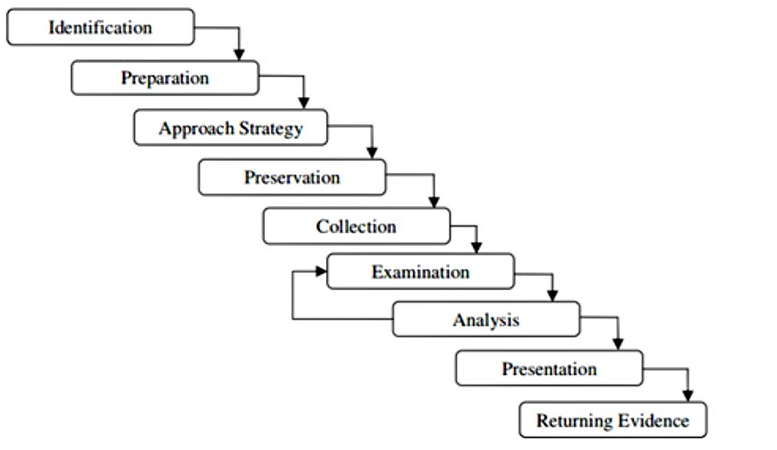
\includegraphics[scale=0.5]{Pictures/DF}
	\par\end{center}

\rule[0.5ex]{0.75\columnwidth}{1pt}

\part{Incident Response:}

Incident Response is an organized approach to addressing and managing
the aftermath of a security breach or cyber-attack.

\section{Incident Response:}

Incident response is a key component of an enterprise business continuity
and resilience program.

The increasing number and diversity of information security threats
can disrupt enterprise business activities and damage enterprise information
assets.

A sound risk management program can help reduce the number of incidents,
but there are some incidents that can neither be anticipated nor avoided.

Therefore, the enterprise needs to have an incident response capability
to detect incidents quickly, contain them, mitigate impact, and restore
and reconstitute services in a trusted manner.

\rule[0.5ex]{0.75\columnwidth}{1pt}

\section{Incident:}
\begin{itemize}
	\item An action likely to lead to grave consequences like,
	\item Data loss may lead to commercial loss.
	\item Confidentiality breached.
	\item Political issues.
	\item Network breakdown lead to service and information flow disruption.
\end{itemize}
\rule[0.5ex]{0.75\columnwidth}{1pt}

\section{Response:}
\begin{itemize}
	\item An act of responding.
	\item Something constituting a reply or a reaction.
	\item The activity or inhibition of previous activity or any of its parts
	      resulting from stimulation
	\item The output of a transducer or detecting device resulting from a given
	      input.
	\item Ideally Incident Response would be a set of policies that allow an
	      individual or individuals to react to an incident in an efficient
	      and professional manner thereby decreasing the likelihood of grave
	      consequences.
\end{itemize}
\rule[0.5ex]{0.75\columnwidth}{1pt}

\section{ISO 17799}
\begin{itemize}
	\item Outlines Comprehensive Incident Response and Internal Investigation
	      Procedures
	\item Detailed Provisions on Computer Evidence Preservation and Handling
\end{itemize}
\rule[0.5ex]{0.75\columnwidth}{1pt}

\section{Purpose of Incident Response:}
\begin{itemize}
	\item Minimize overall impact.
	\item Hide from public scrutiny.
	\item Stop further progression.
	\item Involve Key personnel.
	\item Control situation.
\end{itemize}

\subsection{Minimize overall impact through,}
\begin{itemize}
	\item Recover Quickly \& Efficiently.
	\item Respond as if going to prosecute.
	\item If possible replace system with new one.
	\item Priority one, business back to normal.
	\item Ensure all participants are notified.
	\item Minimize overall impact.
	\item Recover Quickly \& Efficiently.
	\item Secure System.
	\item Lock down all known avenues of attack.
	\item Assess system for unseen vulnerabilities.
	\item Implement proper auditing.
	\item Implement new security measures.
	\item Follow-up (A continuous process)
	\item Ensure that all systems are secure.
	\item Continue prosecution.
	\item Securely store all evidence and notes.
	\item Distribute lessons learned.
\end{itemize}

\subsection{Identifying False Positives:}

Each event that detection tools generate falls into one of four categories,
depending on whether alert fired and whether something bad actually
happened:

\subsubsection{TRUE POSITIVES: Something bad happened, and the system caught it.}

\subsubsection{TRUE NEGATIVES: The activity is benign (gentle, kind), and no alert
	has been generated.}

\subsubsection{FALSE POSITIVES: The system alerts, but the activity was not actually
	malicious.}

\subsubsection{FALSE NEGATIVES: Something bad happened, but the system did not catch
	it.}

Tools do not always alert when something bad happens, and just because
they throw an alarm does not necessarily mean it is time to isolate
a host or call the police.

Example:

Just because an IDS alerted that ``the Web server has been hacked''
does not mean that the Web server was actually hacked.

\rule[0.5ex]{0.75\columnwidth}{1pt}

\section{Signal to Noise Ratio:}
\begin{quotation}
	\noindent \begin{center}
		\textcolor{red}{\LARGE{}EVERY ALERT IS IMPORTANT}{\LARGE\par}
		\par\end{center}
	\begin{center}

		\par\end{center}
\end{quotation}

\subsection{To illustrate, consider the case of SOC A and SOC B.}

In SOC A, the daily work queue contains approximately 100 reliable,
high-fidelity, usable alerts. Each one is reviewed by an analyst.
If incident response is necessary for a given alert, it is performed.

In SOC B, the daily work queue contains approximately 1,00,000 alerts,
almost all of which are false positives. Analysts attempt to review
them according to priority.

Because of the large volume (even for alerts of the highest priority),
analysts cannot successfully review all of the highest-priority alerts.

Additionally, because of the large number of false positives, SOC
B's analysts become desensitized to alerts and do not take them particularly
seriously.

\rule[0.5ex]{0.75\columnwidth}{1pt}

\section{Triage:}

The triage process happens between the moment when an alert is triggered
and the time when an incident response process is initiated.

Not every alert generated by a SIEM product triggers an incident,
some might prompt refinements of SIEM content or changes in security
policy.

This process should include steps that allow security personnel to
unambiguously determine whether the alert is an indicator of an incident,
needs to be suppressed in the future, or requires further investigation
or escalation.

Triage is the assessment of a security event to determine if there
is a security incident its priority and the need for escalation.

As it relates to potential malware incidents the purpose of triaging
may vary.

A few potential questions triaging may address are:
\begin{itemize}
	\item Is malware present on the system?
	\item How did it get there?
	\item What was it trying to accomplish?
\end{itemize}
\rule[0.5ex]{0.75\columnwidth}{1pt}

\section{Security Incident:}

Understanding whether an event is an actual incident is not very simple
and evident every time.

\paragraph{\textcolor{red}{Event Correlation.}}

\paragraph*{Here are a few tips for the verification:}
\begin{itemize}
	\item Adjacent Data -- Check the information adjacent to the event. For
	      example, if an endpoint has a virus signature hit, look to see if
	      there's evidence the virus is running before calling for further
	      response metrics.
	\item Intelligence Review -- Understand the context around the intelligence.
	      Just because an IP address was flagged as part of a botnet last week
	      does not mean it still is part of a botnet today.
	\item Initial Priority -- Align with operational incident priorities and
	      classify incidents appropriately. Make sure the right level of effort
	      is applied to each incident.
	\item Cross Analysis -- Look for and analyse potentially shared keys, such
	      as IP addresses or domain names, across multiple data sources for
	      better data acuity.
\end{itemize}

\paragraph{Once an event is verified, the event becomes an investigation or
	an incident. All incidents must be investigated and tracked.}

\rule[0.5ex]{0.75\columnwidth}{1pt}

\section{Classification of Types of Incidents:}

Understand what types of attacks are likely to be used against your
organization.

List of different attach by NIST is:

\subsubsection{External/Removable Media: An attack executed from removable media
	(e.g., flash drive, CD) or a peripheral device.}

\subsubsection{Email: An attack executed via an email message or attachment (e.g.
	malware infection).}

\subsubsection{Attrition: An attack that employs brute force methods to compromise,
	degrade, or destroy systems, networks, or services. }

\subsubsection{Improper Usage: Any incident resulting from violation of an organization\textquoteright s
	acceptable usage policies by an authorized user, excluding the above
	categories.}

\subsubsection{Web: An attack executed from a website or a web-based application
	(e.g. drive-by download).}

\subsubsection{Loss or Theft of Equipment: The loss or theft of a computing device
	or media used by the organization, such as a laptop or smartphone.}

\subsubsection{Other: An attack that does not fit into any of the other categories.}

\rule[0.5ex]{0.75\columnwidth}{1pt}

\section{Action on Security Incident:}

\subsection{Incident Scene Snapshot:}
\begin{itemize}
	\item Record state of computer
	\item Photos,
	\item State of computer,
	\item What is on the screen?
	\item What is obviously running on the screen?
	\item Xterm?
	\item X-windows?
	\item Should you port scan the affected computer?
\end{itemize}
\begin{description}
	\item [{Pros:}] You can see all active and listening ports.
	\item [{Cons:}] It affects the computer and some backdoor log how many
	      connections come into them and could tip off the bad guy.
\end{description}

\subsection{Unplug Power from System:}

\paragraph{This method may be the most damaging to effective analysis though
	there are some benefits.}
\begin{description}
	\item [{Pros:}] Benefits include that you can now move the system to a
	      more secure location and that you can physically remove the hard drive
	      from the system
	\item [{Cons:}] You lose evidence of all running processes and memory.
\end{description}

\subsection{Unplug from The Network:}
\begin{itemize}
	\item Unplug it from the network and plug the distant end into a small hub
	      that is not connected to anything else.
	\item Most systems will write error messages into log files if not on a
	      network.
	\item If you make the computer think it is still on a network, you will
	      succeed in limiting the amount of changes to that system.
\end{itemize}

\subsection{Backup or Analyse:}

\paragraph{Set up in policy for your incident response:}
\begin{itemize}
	\item It depends on the system and what you need it for.
	\item To get BEST evidence BACKUP first at the cost of time to get answers.
	\item To get FAST answers ANALYSE first at the cost of getting best evidence.
	\item Label systems with priority. Some will need answers quicker than your
	      ability to get best evidence.
\end{itemize}
\rule[0.5ex]{0.75\columnwidth}{1pt}

\section{Prioritizing Incidents:}
\begin{itemize}
	\item An Incident's priority is usually determined by assessing its impact
	      and urgency.
	\item Urgency is a measure how quickly a resolution of the Incident is required.
	\item Impact is measure of the extent of the Incident and of the potential
	      damage caused by the Incident before it can be resolved.
\end{itemize}
\rule[0.5ex]{0.75\columnwidth}{1pt}

\pagebreak{}

\section{Incident Prioritizing Table:}
\begin{center}
	\begin{tabular}{|c||l|}
		\hline
		\textbf{CATEGORY}                                            & \textbf{DESCRIPTION}\tabularnewline
		\hline
		\hline
		\multirow{4}{*}{\textbf{\textcolor{red}{\Large{}HIGH}}}      & The damage caused by the incident increases rapidly. \tabularnewline
		\cline{2-2}
		                                                             & Work that cannot be completed by the staff is highly time sensitive.\tabularnewline
		\cline{2-2}
		                                                             & A minor incident can be prevented from becoming a major incident by
		acting immediately.\tabularnewline
		\cline{2-2}
		                                                             & Several users with VIP status are affected.\tabularnewline
		\hline
		\multirow{2}{*}{\textbf{\textcolor{orange}{\Large{}MEDIUM}}} & The damage caused by the incident increases considerably over time. \tabularnewline
		\cline{2-2}
		                                                             & A single user with VIP status is affected. \tabularnewline
		\hline
		\multirow{2}{*}{\textbf{\textcolor{teal}{\Large{}LOW}}}      & The damage caused by the incident only marginally increases over time. \tabularnewline
		\cline{2-2}
		                                                             & Work that cannot be completed by staff is not time sensitive.\tabularnewline
		\hline
	\end{tabular}
	\par\end{center}
\end{document}
